%
% File emnlp2016.tex
%

\documentclass[11pt,letterpaper]{article}
\usepackage{emnlp2016}
\usepackage{times}
\usepackage{latexsym}
\usepackage{hyperref}
\usepackage{graphicx}
\graphicspath{ {../plots/} }
\usepackage{subcaption}
\usepackage[font=footnotesize,labelfont=bf]{caption}
\usepackage{multirow}

% Uncomment this line for the final submission:
\emnlpfinalcopy

% To expand the titlebox for more authors, uncomment
% below and set accordingly.
% \addtolength\titlebox{.5in}    

\newcommand\BibTeX{B{\sc ib}\TeX}
\newcommand{\code}[1]{\texttt{#1}}


\title{HW2: Part-of-Speech Tagging with LSTMs}

\author{Pratyush Kar\\
  {\tt UT EID: pk8498}}

\date{}

\begin{document}

\maketitle

\begin{abstract}
  Part-of-Speech (POS) tagging is the lowest form of syntactic analysis of text. POS tags are useful for subsequent syntactic parsing and word sense disambiguation. POS tagging is a classic example of a sequence labelling task and Bidirectional Long Short Term Memory networks (Bi-LSTMs) can be applied to this problem. In this experiment, we extract orthographic features from each word, and investigate the effects of adding these features during training, on the predictive and run-time performance of the network. We also compare how different network architectures affects the out-of-vocabulary (OOV) accuracy of model.
\end{abstract}

\section{Introduction}
A Part-of-Speech tagger is a software that reads natural language text and assigns each word an appropriate part of speech such as noun, verb, adverb etc. It is the lowest level of syntactic analysis and is useful for subsequent higher level tasks in the NLP pipeline like parsing and WSD. Since, the tag of any word depends on its context, this problem can be modelled as a sequence labelling problem. LSTMs have been known to be good for these kinds of problems. Bi-LSTMs are an extension of the LSTM networks but, instead of processing the sequence in only the forward direction, they model the sequence in both forward and backward directions. Bi-LSTMs are comprised of two LSTMs a forward and backward LSTM which process the input sequence in the forward and backward direction respectively. The output of the Bi-LSTM is just the concatenation of the outputs of the forward and backward LSTMs. Due to this reason they generally perform better on sequence labelling tasks because they can encode context from both the directions.

\section{Model and Dataset}
In this experiment, we use the WSJ data from the Penn Treebank. We use the standard splits for the WSJ dataset which partitions the dataset into 80:10:10 splits for training, validation and test sets respectively. The dataset is preprocessed before training the model. The training set is used to generate the vocabulary of the model and the words in the sequences are replaced by the word identifier using this vocabulary. Out-of-vocabulary (OOV) words in validation and test sets are replaces with a unique \code{<UNK>} token. All sequences are padded to have uniform length (\code{MAX\_LENGTH}). All sentences that are longer than \code{MAX\_LENGTH} are dropped. In order to make the training of the Bi-LSTM tractable, the word identifiers are replaced with the a linear word embedding. The word ids are used to index into this embedding matrix and the embedding is used as the input to the network. This embedding is also learned during the training of the Bi-LSTM network.

The model is trained for 700 epochs. To speed up training and accurately estimate the gradient we give the training examples to the network in batches of size 128. After every 10 epochs the model is tested on the validation set and model accuracy and the OOV accuracy is recorded. The validation set is used to prevent overfitting and identify the model that generalizes the best.

\begin{figure*}[htbp]
	\centering
	\captionsetup{justification=centering}
	\begin{subfigure}[b]{0.48\textwidth}
		\centering
		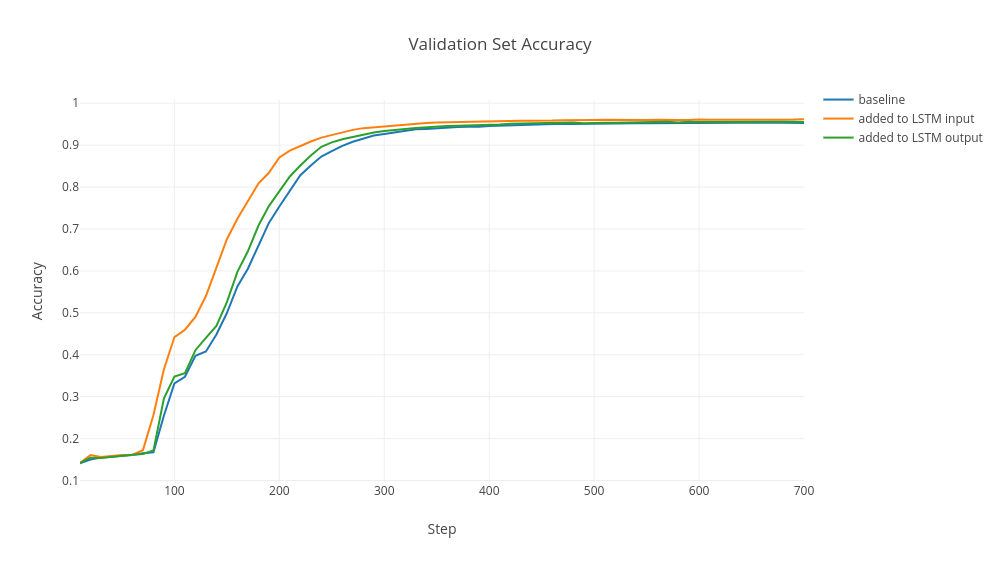
\includegraphics[width=\linewidth]{Validation-Accuracy}
		\caption{Validation set accuracy}
		\label{a}
	\end{subfigure}
	\centering
	\begin{subfigure}[b]{0.48\textwidth}
		\centering
		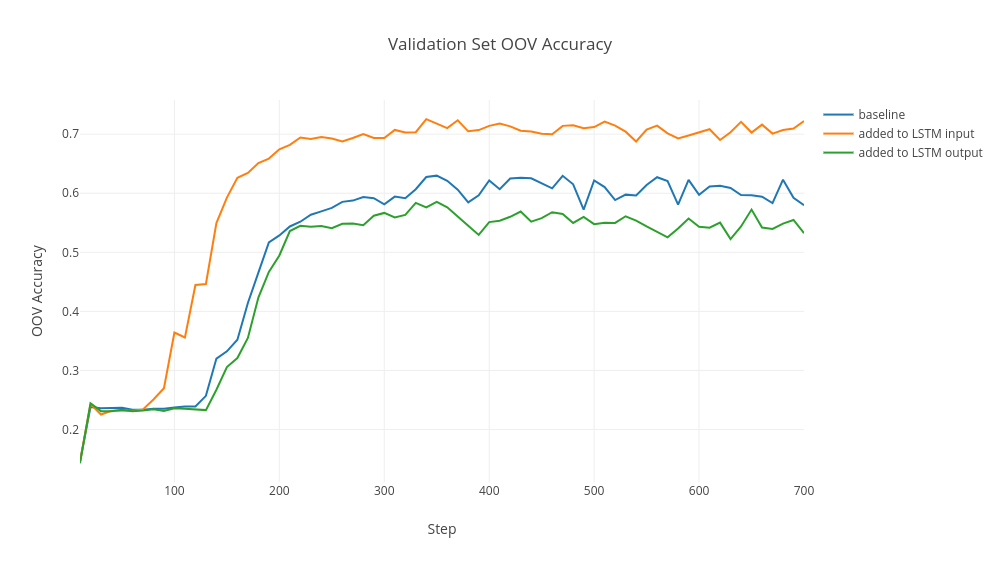
\includegraphics[width=\linewidth]{Validation-OOV-Accuracy}
		\caption{Validation set OOV accuracy}
		\label{b}
	\end{subfigure}
	\caption{The validation set accuracy was measured at regular intervals of 10 epochs. The blue line represents the results for the baseline model (without any orthographic features). Orange and green lines represent the results of the model when the orthographic word features were added to the LSTM input and output respectively.}
	\label{fig:graphs}
\end{figure*}

\section{Orthographic Features}
One limitation in the baseline model is the way it handles the OOV words. Irrespective of the words present in the text, all OOV words are given the same embedding vector. This gives the network very little information to accurately tag these OOV words. It only has the context of the word for predicting the POS tag. In most OOV cases, little information about the structure of the word itself is enough to predict the POS tag correctly. For example, if an OOV words starts with a capital letter it is highly likely that this word is a proper noun. POS tags can be divided into 2 types -- open and closed classes \footnote{Prof. Ray Mooney's lecture on Part-of-Speech tagging \url{https://www.cs.utexas.edu/~mooney/cs388/slides/pos-tagging.ppt}.}. Closed classes are composed of a small, fixed set of grammatical function words for example pronouns, prepositions, determiners, particles, conjunctions, etc. These categories typically are fixed for a given language. New words in these classes are hard to come by. Open classes on the other hand have large number of words and new words can easily be invented. Nouns are the most common kind of open class part of speech. For such words, even little information about the structure of the word itself is enough to accurately identify their POS tags.

Orthographic features of a word are observational features related to the structure of the word itself. In our experiments, we use 5 kinds of orthographic features -- capitalized first letter, word has hyphen, starts with a number, word suffixes and word prefixes. We consider 4 different types of suffixes based on their part of speech -- noun suffixes like \emph{-ism} (eg. Judaism), verb suffixes like \emph{-ate} (eg. mediate), adjective suffixes like \emph{-ible} (eg. edible) and adverb suffixes like \emph{-ly} (eg. slowly). Unlike suffixes, prefixes are not directly related to their part-of-speech classes but even then we thought that adding prefixes might be useful. Although there is no direct relation between the prefix and the POS tag there is a correlation in some cases, for eg. \emph{dis-} typically shows up in verbs like \emph{disagree, displeasure, disqualify}. In total we consider 39 suffixes and 31 prefixes. For a full list of the prefixes and suffixes considered, please see \code{orth\_feats.py} which gives a detailed description. For each word, the orthographic features are computed as a one-hot vector where the vector entry is 1 if the respective feature is present otherwise the entry is 0.

\subsection{LSTM Architecture Changes}

\begin{table*}[t]
\centering
\caption{Experiment Results}
\label{table:results}
\begin{tabular}{c|ccc|cc|c}
\multirow{2}{*}{Model} & \multicolumn{3}{c|}{Accuracy}                           & \multicolumn{2}{c|}{OOV Accuracy}   & \multirow{2}{*}{\begin{tabular}[c]{@{}c@{}}Training Runtime\\ (approx. min)\end{tabular}} \\
                       & train             & val              & test             & val              & test             &                                                                                           \\ \hline
baseline               & 0.9764            & 0.953            & 0.955            & 0.532            & 0.520            & \textbf{30}                                                                             \\
added to LSTM input       & 0.9766            & \textbf{0.962} & \textbf{0.963} & \textbf{0.722} & \textbf{0.728} & 58                                                                                        \\
added to LSTM output      & \textbf{0.9790} & 0.955            & 0.956            & 0.580            & 0.562            & 57              
\end{tabular}
\end{table*}

We also need to change the Bi-LSTM architecture for adding the orthographic word features. There are two different ways in which these orthographic features can be added to the network. The features can either be concatenated to the word embedding and given to the Bi-LSTM as input or they can be concatenated to the output of the Bi-LSTM before passing to the linear classification layer. We consider both implementations in our experiments. We also add the implementation to calculate the OOV accuracy for the validation set. This is done by computing a mask for the OOV words in the sequence. The accuracy for the entire batch is then calculated normally using the model probabilities and output tags. This is then multiplied by the OOV word mask. The total OOV accuracy is divided by the number of OOV words in the sequence to compute the average OOV accuracy.

\section{Results}
All three models, baseline and the two LSTM architectures (with orthographic features), are trained on the training set of WSJ dataset. The results for the three models are reported in Table \ref{table:results}. OOV accuracy for the training set is not defined hence, it is only reported for the test and validation set. For computational reasons the training was stopped when the accuracy on the validation set did not change substantially. For all the models it can be seen in Fig. \ref{fig:graphs} that the validation set accuracy converges around epoch 600.

\subsection{Baseline vs. Bi-LSTM with orthographic features}
Although the vanilla Bi-LSTM model gives a POS tag accuracy of 95.5\% accuracy on the overall test set it fails to perform on the OOV words where it gets an accuracy of 53.2\%. This is primarily because of the way the baseline model handles OOV words. All OOV words are given the same embedding vector irrespective of the word present in the text. The network has to predict the POS tag based only on the context of the word which can be very ambiguous. On the other hand adding the word orthographic features to the input of the network raises the OOV accuracy to 72.8\% and test accuracy to 96.3\%.

As discussed before, the OOV words are generally in the open class of POS tags like nouns, verbs, adjectives, adverbs, etc. Open classes have large number of words and new words can easily be invented. Such words sometimes have distinct features like proper nouns always start with a capital letter, adverbs end with \emph{-ly}, etc. Hence, adding orthographic features, that capture such patterns, allow the network to identify these words successfully even though it has never seen them during the training phase. Another interesting thing to note here is that, even though OOV accuracy on the test set increases substantially ($\sim16.6\%$), the total accuracy increases only by a small margin ($\sim0.8\%$). This is because the OOV words form a very small proportion ($\sim2.74\%$) of the test set.

\subsection{Runtime Comparison}
The models were run on a Late 2013 MacBook Pro with a 2.3 GHz Intel Core i7 processor. Only CPU was used for running the models. Vanilla Bi-LSTM without the orthographic features trained in almost half the time of the Bi-LSTMs with orthographic features (see Table \ref{table:results}). This is because of the increase in the size of the tensors in the network. A portion of the increase in the time can also be attributed to the additional computation required to calculate the orthographic features of the words.

\subsection{Adding Features to Input Layer vs. Classification Layer}
We consider 2 different network architectures -- one in which features are concatenated to the word embedding and given to the Bi-LSTM as input, in the other they are concatenated to the output of the Bi-LSTM before passing it to the linear classification layer. Based on the results (in Table \ref{table:results}) we can observe that the Bi-LSTM where the features are concatenated to the LSTM input perform substantially better than its counterpart in both the test set accuracy and test set OOV accuracy. This is largely due to the presence of input, output and forget gates present in the LSTM architecture. In the latter case there is only a single linear layer before the predictions are made. That linear layer can only learn a very simple linear function which makes it very difficult for it to fit complex functions. LSTM on the other hand can choose to add only the relevant information to its internal cell state and using that it can output the appropriate information required to make the prediction. It is possible that most of the orthographic features may be irrelevant to predicting a given words POS tag. In that case an LSTM can choose to encode only the relevant information in its cell state and use this to predict the correct tag hence, it performs better.

If we compare the plots of the models in Fig. \ref{a}, we can see that the LSTM with features added to the input layer converges faster than its counterparts. This suggests that adding the orthographic features to the input of the LSTM somewhat accelerates its learning even though there is not much difference final validation set accuracies.

\section{Conclusion}
POS tagging is one of the most studied problems in natural language processing. Simple stochastic models like HMMs have been able to achieve accuracies of around $~96\%$\footnote{ACL Wiki POS Tagging (State of the art) \url{https://aclweb.org/aclwiki/POS_Tagging_(State_of_the_art)}}. Bi-LSTMs also perform exceedingly well on this problem but don't perform that well on OOV words. Based on our results it is evident that adding orthographic word features to the input of the LSTM increases OOV accuracy substantially and accelerates the learning process. 

\end{document}
